\documentclass[10pt,twocolumn,letterpaper]{article}

\usepackage{cvpr}
\usepackage{times}
\usepackage{epsfig}
\usepackage{graphicx}
\usepackage{amsmath}
\usepackage{amssymb}
\usepackage{svg}
\usepackage{currfile}
\usepackage{minibox}

\usepackage[breaklinks=true,bookmarks=false]{hyperref}

\cvprfinalcopy

\def\cvprPaperId{****}
\def\httilde{\mbox{\tt\raisebox{-.5ex}{\symbol{126}}}}

\setcounter{page}{1}
\begin{document}

\title{ Exploiting synthetic images for real-world image recognition }

\author{Max Maton\\
Delft University of Technology\\
Delft, The Netherlands\\
{\tt\small https://in.maxmaton.nl/}
\and
Jan van Gemert\\
Delft University of Technology\\
Delft, The Netherlands\\
{\tt\small http://jvgemert.github.io/}
\and
Miriam Huijser\\
Aiir Innovations\\
Amsterdam, The Netherlands\\
{\tt\small https://aiir.nl/}
\and
Osman Kayhan\\
Delft University of Technology\\
Delft, The Netherlands\\
{\tt\small o.s.kayhan@tudelft.nl}
}

\maketitle

\iffalse
Abstract
</h2>
<p>
\fi

\begin{abstract}

This paper shows that the gap between synthetic and real-world image distributions can be closed by using GANs to convert the synthetic data to a dataset which has the same distribution as the real data. Training this GAN requires only a fraction of the dataset traditionally required to get a high classification accuracy. This converted data can subsequently be used to train a classifier with a higher accuracy than a classifier trained only on the real dataset.

\end{abstract}

\iffalse
<h2>
Introduction
</h2>
<div class="figure" id="figure1">
<img src="method.svg" width="300em"><br>
Figure 1. <i>Technique used to convert synthetic dataset to be used in training.</i>
</div>

<p>
\fi

\begin{figure}[h]
\begin{center}
\fbox{\rule{0pt}{2in} %\rule{0.1\linewidth}{0pt}%
   {\scriptsize \includesvg[width=0.85\linewidth]{../method.svg}}%
}
\end{center}
   \caption{Technique used to convert synthetic dataset for use in training.}
\label{fig:method}
\end{figure}

\section{Introduction}

Deep learning has revolutionised visual object recognition. Thanks to huge datasets and fast hardware (GPUs), current object recognition approaches have near-human accuracy.
%<p>
Because creating big datasets is often very expensive, people are starting to turn to synthetic images to augment their datasets. However, training networks on synthetic images may not achieve the desired accuracy due to a gap between synthetic and real image distributions. \cite{10.1.1.151.7688}
%<p>
Another development is the increased focus on Generative Adversarial Networks (GANs) to generate images that look similar to the images they were trained on. \cite{1406.2661}
%<p>
In this paper the impact of the distribution gap between synthetic and real image distributions is decreased by using a GAN to modify the synthetic images to have the same distribution as real images. This technique is shown to be useful for inflating very small datasets to a level where they can be used to create accurate classifiers.

\iffalse
<h2>
Related work
</h2>
<p>
\fi

\section{Related work}
Artificial data can sometimes be used to train networks, i.e. a network trained on rendered images to segment images of indoor scenes \cite{10.1.1.94.777}, a network that recognises font characters trained on interpolated real samples \cite{10.1.1.151.7688} and a network trained with simulations to train control networks. \cite{10.1109/CVPR.2016.442} These networks are trained by creating a synthetic dataset that is as close as possible in statistical distribution as the real dataset. Generally this is very difficult or expensive to achieve.

%<p>
A solution for the problem of creating synthetic datasets with a distribution close to a real dataset is domain adaptation. This is generally done using Generative Adversarial Networks \cite{1703.05192.pdf, 10.1109/CVPR.2017.18, 10.1007/978-3-319-58347-1} that are trained to create samples that are indistinguisable from images in the real dataset based on images in the crude synthetic dataset. We decided to perform this research on the GAN as described by Bousmalis et al \cite{10.1109/CVPR.2017.18} due to the available TensorFlow \cite{tensorflow} implementation.

%<p>
The problem of creating synthetic datasets with a distribution close to a real dataset can be solved by using domain adaptation. This is generally done using Generative Adversarial Networks \cite{1703.05192.pdf, 10.1109/CVPR.2017.18, 10.1007/978-3-319-58347-1} ttrained to create samples based on images in the crude synthetic dataset that are indistinguisable from images in the real dataset. We decided to perform this research on the GAN as described by Bousmalis et al \cite{10.1109/CVPR.2017.18} due to the available TensorFlow \cite{tensorflow} implementation.



\iffalse
<h2>
Inflating datasets using synthetic data and GANs
</h2>
<p>
\fi

\section{Inflating datasets using synthetic data and GANs}

The basis of this research is the GAN that converts images from a synthetic dataset distribution to an image that appears to come from the distribution of a real dataset. This GAN consists of three parts. The first part is a generator network that does the image conversion. The second part of the GAN is a discriminator, which tries to distinguish between the output of the generator and images from the real dataset. The third part of the GAN is a classifier that predicts the label of images coming from either the real dataset, the generator or the synthetic dataset. All these networks are trained in parallel. The discriminator and classifier are trained to reduce the amount of misclassifications. The generator is trained to minimise the amount of pixels changed in the image, to minimise the loss in classification by the classifier and to try to fool the discriminator to classify the image as real.

%<p>
To test the effects of inflating datasets when using this technique, we first trained the GAN with a real and synthetic dataset. We then use the trained GAN to create a new dataset and combine that dataset with the real dataset. This combined dataset is then used to train a second classifier.

\subsection{Experiments}


We evaluated this technique on the MNIST dataset \cite{mnist} together with a synthetic dataset generated by rendering open source font digits in multiple rotations for all number classes.
%<p>
The synthetic dataset contains samples from $149$ fonts, with each digit rendered having $47$ variations each with a distinct rotation between $-47$ and $46$ degrees. All images were normalised using the same algorithm used to normalise the MNIST samples, the result of which can be seen in figure \ref{fig:example-font-images}. A random sample of $10,030$ of those images were put in a test set and the remaining $60,000$ images were used as the synthetic dataset.

\begin{figure}[t]
\begin{center}
\fbox{\rule{0pt}{2in} %\rule{.7\linewidth}{0pt} 
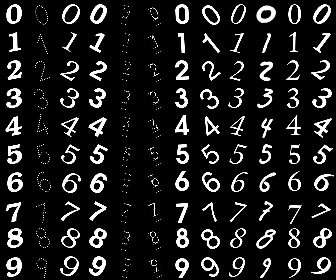
\includegraphics[width=0.8\linewidth]{example-font-images.png}%
}
\end{center}
   \caption{Example images of the MNIST font dataset}
\label{fig:example-font-images}
\end{figure}

%<p>
The GAN was modified to use $10\%$ of the training data as a validation set instead of a constant $1,000$ samples as this allowed for smaller sample sizes.

%<p>
For multiple ratios r, where $0 > r > 1$, we created the following datasets:

\begin{description}
	\item{$\text{MNIST}_\text{original}$} \hfill \\ $60,000 \times r$ images from the original MNIST dataset.
	\item{$\text{MNIST}_\text{font}$} \hfill \\ $60,000 \times (1 - r)$ images from the synthetic font dataset.
\end{description}

%<p>
We used these two datasets to train the GAN using 12 million training samples and subsequently ran the GAN on the $\text{MNIST}_\text{font}$ dataset to create the $\text{MNIST}_\text{GAN}$ dataset. This made the $\text{MNIST}_\text{GAN}$ dataset exactly as big as $\text{MNIST}_\text{font}$.

%<p>

With these datasets we trained five instances of the following classifiers:

\begin{description}
	\item{$5\times \text{C-MNIST}_\text{original}$} \hfill \\ Classifier only trained on $\text{MNIST}_\text{original}$
	\item{$5\times \text{C-MNIST}_\text{font}$} \hfill \\ Classifier only trained on $\text{MNIST}_\text{font}$
	\item{$5\times \text{C-MNIST}_\text{GAN}$} \hfill \\ Classifier only trained on $\text{MNIST}_\text{GAN}$
	\item{$5\times \text{C-MNIST}_\text{original+GAN}$} \hfill \\ Classifier only trained on $\text{MNIST}_\text{original+GAN}$
	\item{$5\times \text{C-MNIST}_\text{original+font}$} \hfill \\ Classifier only trained on $\text{MNIST}_\text{original+font}$
\end{description}

%<p>
Each classifier was tested on the MNIST test set which resulted in an accuracy percentage.

\clearpage

\section{Results}

%<p>
To validate whether the GAN was creating useful images, we looked at the resulting images in $\text{MNIST}_\text{GAN}$:

\begin{figure}[h]
\begin{center}
%\fbox{\rule{0pt}{2in} %\rule{.7\linewidth}{0pt} %
\minibox[frame]{
	\parbox{0.8\linewidth}{ \small $r = 0.001$ } \\
	\parbox{0.8\linewidth}{ 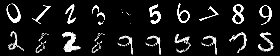
\includegraphics[width=0.8\linewidth]{results-001.png} } \\
	\parbox{0.8\linewidth}{ \small $r = 0.007$ } \\
	\parbox{0.8\linewidth}{ 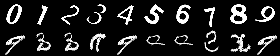
\includegraphics[width=0.8\linewidth]{results-007.png} } \\
	\parbox{0.8\linewidth}{ \small $r = 0.100$ } \\
	\parbox{0.8\linewidth}{ 
\includegraphics[width=0.8\linewidth]{results-100.png} } \\
	\parbox{0.8\linewidth}{ \small $r = 0.700$ } \\
	\parbox{0.8\linewidth}{ 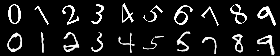
\includegraphics[width=0.8\linewidth]{results-700.png} } \\
}
\end{center}
   \caption{Example images of the MNIST font dataset. Top of each image is from $\text{MNIST}_\text{font}$, bottom is the generated image in $\text{MNIST}_\text{GAN}$ }
\label{fig:results}
\end{figure}

%<p>
From visual inspection it is apparent that the GAN has trouble keeping the labels consistent if there is not enough real training data. An example of this are the 1 and the 2 of $r = 0.007$ in figure \ref{fig:results}: they both result in something that looks like the same 8 instead of something that looks like a 1 or 2 respectively. This means that the classifier trained on this new dataset will receive two very similar samples with conflicting labels. We measured the accuracy on MNIST of $\text{C-MNIST}_\text{GAN}$ and found low accuracy for lower ratios. This supports the conclusion that there is an issue with labeling.

%<p>
We measured the performance of $\text{C-MNIST}_\text{original+GAN}$ versus $\text{C-MNIST}_\text{original}$. It showed that even though the generated samples are not good samples for their target class, $\text{C-MNIST}_\text{original+GAN}$ is much more accurate than $\text{C-MNIST}_\text{original}$. This effect can partially be explained by results shown by Sukhbaatar et al. that indicate that deep learning is robust to massive label noise. \cite{Sukhbaatar2014TrainingCN} This would mean that the network is still capable of learning higher level features from the mislabeled samples and is able to succesfully ignore the bad labeling. This indicates that this technique is succesfully able to close the distribution gap once a lower bound on the amount of available real images has been reached.

\iffalse
<h3>C-MNIST<sub>font</sub> performance</h3>
<div class="figure" id="figure4">
<img src="graph-font.png" width="90%"><br>
Figure 4. <i>Performance of C-MNIST<sub>font</sub> with varying amounts of MNIST<sub>font</sub> training data. Performance decreases with more training samples indicating that MNIST<sub>original</sub> and MNIST<sub>font</sub> have different characteristics.</i>
</div>
<p>
\fi

\subsection{$\text{C-MNIST}_\text{font}$ performance}
\begin{figure*}
\begin{center}
\fbox{\rule{0pt}{2in} %\rule{.7\linewidth}{0pt} %
	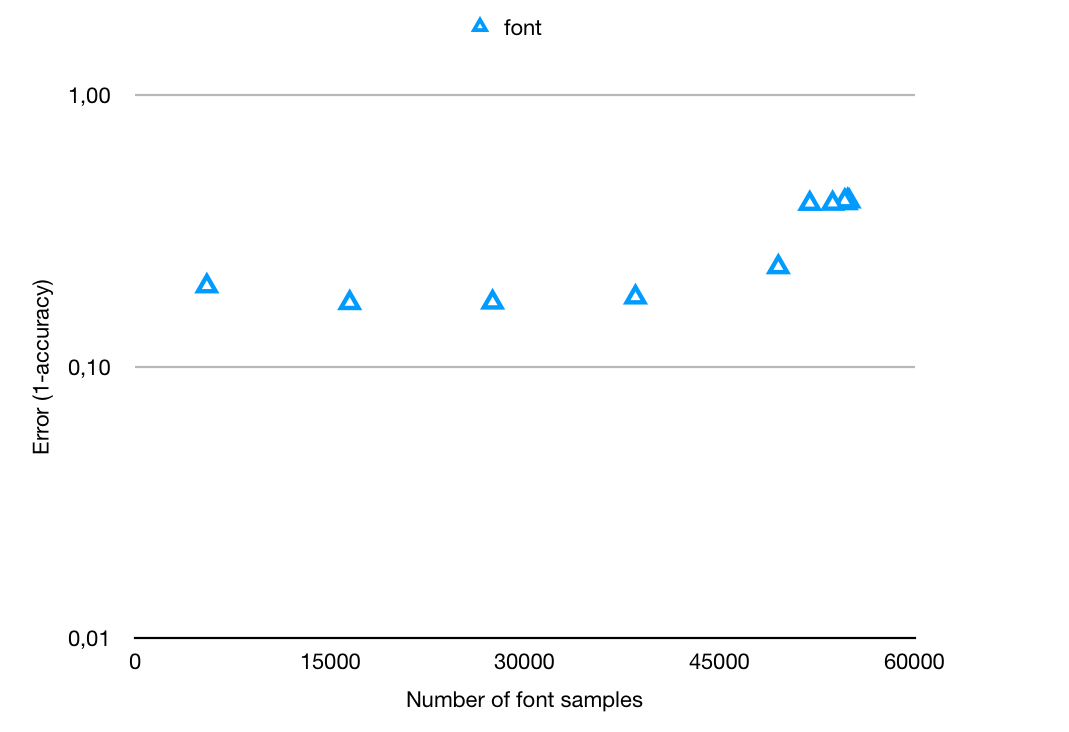
\includegraphics[width=0.8\linewidth]{../graph-font.png}
}
\end{center}
   \caption{Performance of $\text{C-MNIST}_\text{font}$ with varying amounts of $\text{MNIST}_\text{font}$ training data. Performance decreases with more training samples indicating that $\text{MNIST}_\text{original}$ and $\text{MNIST}_\text{font}$ have different characteristics}
\label{fig:graph-font}
\end{figure*}

To make sure we actually test whether the GAN is able to close the distribution gap we looked at the accuracy of $\text{C-MNIST}_\text{font}$. For this dataset the error shows an inverse relation between the amount of samples and the performance of the classifier as can be seen in figure \ref{fig:graph-font}. This indicates that a gap exists between the raw font dataset and the MNIST test dataset.

\iffalse
<h3>
Classifier performance
</h3>
<div class="figure" id="figure5">
<img src="graph-results.png" width="90%"><br>
Figure 5. <i>Performance of classifiers with different amounts of MNIST training data. Training with the GAN data improves results after a minimal amount of original MNIST samples.</i>
</div>
\fi


\subsection{Classifier performance}
\begin{figure*}
\begin{center}
\fbox{\rule{0pt}{2in} %\rule{.7\linewidth}{0pt} %
	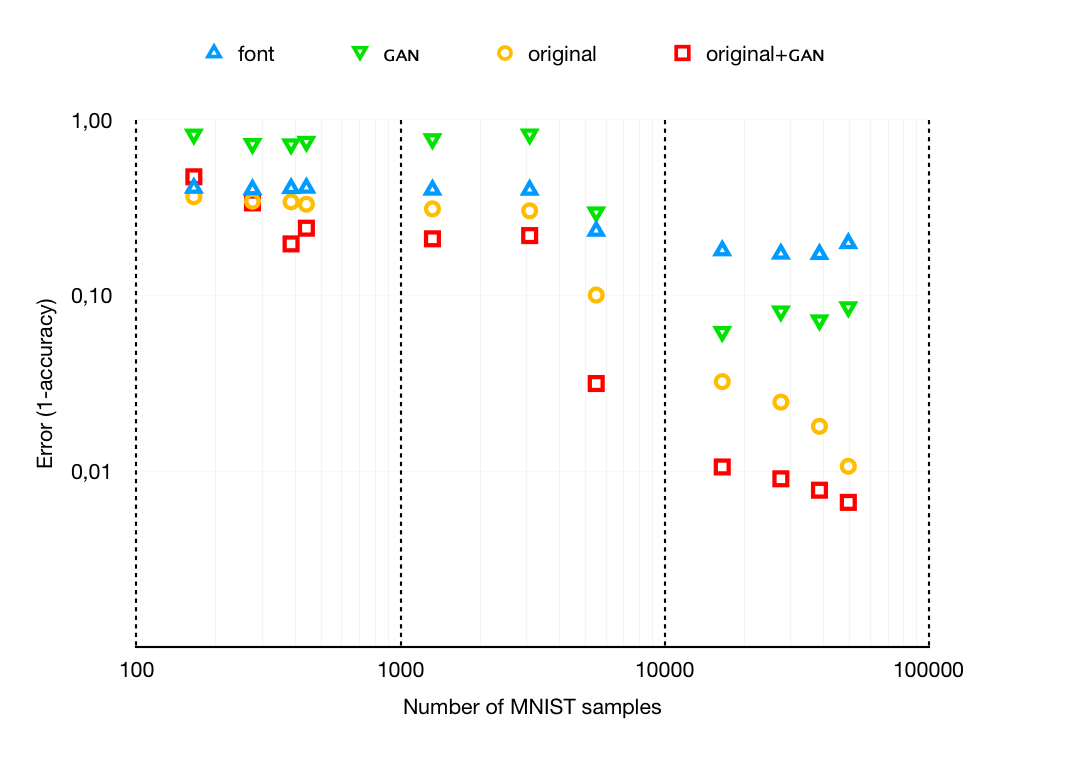
\includegraphics[width=0.8\linewidth]{../graph-results.png}
}
\end{center}
   \caption{Performance of classifiers with different amounts of MNIST training data. Training with the GAN data improves results after a minimal amount of original MNIST samples}
\label{fig:graph-results}
\end{figure*}

%<p>
We compared the accuracy of $\text{C-MNIST}_\text{font}$, $\text{C-MNIST}_\text{GAN}$, $\text{C-MNIST}_\text{original}$ and $\text{C-MNIST}_\text{original+GAN}$ to see whether training with the $\text{MINST}_\text{original+GAN}$ dataset is better than training with one of the individual datasets. The result of this comparison can be seen in figure \ref{fig:graph-results}.

%<p>
There seems to be a minimum amount of real samples after which the GAN starts to produce meaningful data. In this case $\text{C-MNIST}_\text{original+GAN}$ is only more accurate than the $\text{C-MNIST}_\text{original}$ when the GAN is trained on more than 385 real images ($r = 0.007$).

%<p>
Using MNIST as a test case, this technique is able to close the distribution gap even with as little $0.7\%$ real data in the resulting dataset.

\iffalse
<h3>C-MNIST<sub>original</sub> against C-MNIST<sub>original+font</sub></h3>

<div class="figure" id="figure6">
<img src="graph-font-original-comparison.png" width="90%"><br>
Figure 6. <i>Performance of C-MNIST<sub>original+font</sub> versus the performance of C-MNIST<sub>original</sub> for varying amounts of training data. Performance is almost the same indicating no advantage to including font data in the training set directly.</i>
</div>
\fi

\subsection{$\text{C-MNIST}_\text{original}$ against $\text{C-MNIST}_\text{original+font}$}
\begin{figure*}
\begin{center}
\fbox{\rule{0pt}{2in} %\rule{.7\linewidth}{0pt} %
	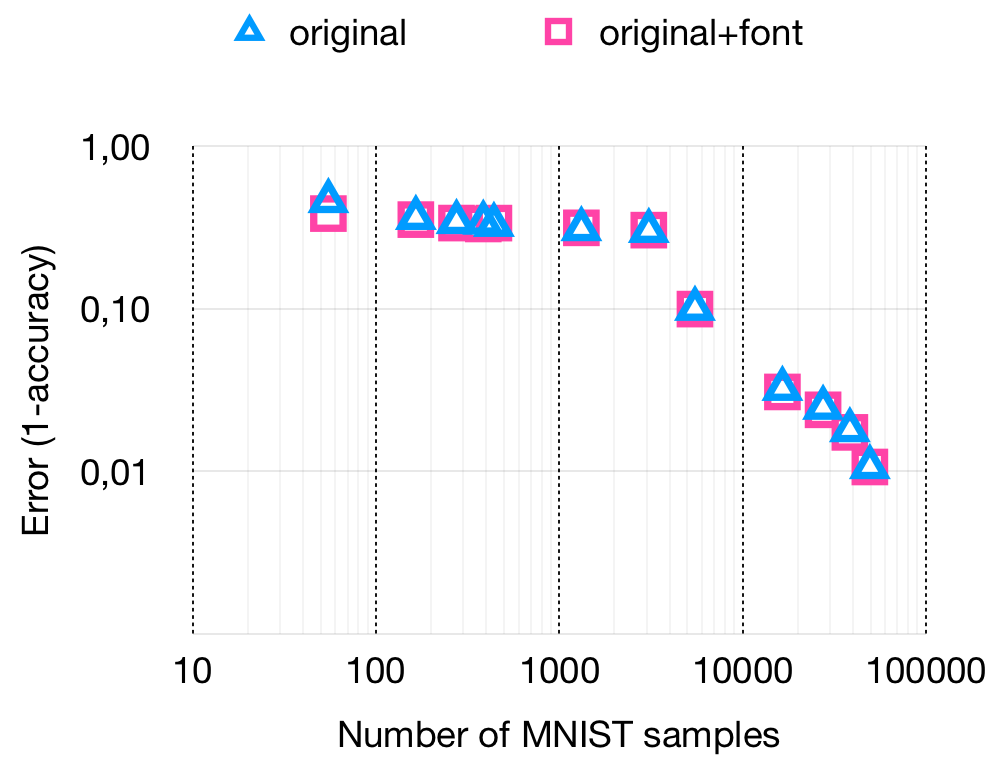
\includegraphics[width=0.8\linewidth]{../graph-font-original-comparison.png}
}
\end{center}
   \caption{Performance of $\text{C-MNIST}_\text{original+font}$ versus the performance of $\text{C-MNIST}_\text{original}$ for varying amounts of training data. Performance is almost the same indicating no advantage to including font data in the training set directly.}
\label{fig:graph-font-original-comparison}
\end{figure*}

%<p>
To confirm that the improved results of $\text{C-MNIST}_\text{original+GAN}$ can not be solely explained by the addition of more data, we compared $\text{C-MNIST}_\text{original}$ with $\text{C-MNIST}_\text{original+font}$ to see if the addition of font data increased the accuracy. From the results in figure \ref{fig:graph-font-original-comparison} we had to conclude that $\text{C-MNIST}_\text{original+font}$ has performance roughly equal to $\text{C-MNIST}_\text{original}$ and therefore cannot explain the additional accuracy of $\text{C-MNIST}_\text{original+gan}$.

\iffalse
<h2>
Discussion
</h2>
<p>
\fi

\section{Discussion}

Due to a limited amount of time, no optimization has been done on the hyperparameters of the GAN. Optimizing these hyperparameters might further improve classification accuracy which should result in a further reduction in the amount of required samples from the real dataset.

\iffalse
<h2>
Conclusion
</h2>
<p>
\fi

\section{Conclusion}

Using MNIST as an example, we were able to show that it's possible to create a synthetic dataset. We've shown that a distribution gap exists between the dataset we created and the real MNIST dataset and were able to close this gap using our described technique.

%<p>
We've shown that GANs can be used to inflate trainingsets by reducing the gap between synthetic and real datasets. Furthermore, they can do so with very little real training data.

{\small
\bibliographystyle{ieee}
\bibliography{references}
}

\iffalse
</body>
</html>
\fi
\end{document}
